\documentclass[11pt, twoside]{report}
\usepackage[utf8]{inputenc}
\usepackage[margin=2.5cm]{geometry}
\usepackage{graphicx}  		% display images
\usepackage{rotating}
\usepackage{tikz} 
\usepackage[portuguese]{babel}
\usepackage{indentfirst}
\usepackage[colorlinks=true,linkcolor=black,urlcolor=black,bookmarksopen=true]{hyperref} % Make hyperlinks in index
\usepackage{bookmark} 		% Bookmarks for pdf file
\usepackage{float} 			% colocar as imegens e tabelas dentro do texto
\usepackage{fancyhdr}
\pagestyle{fancy}
\usepackage{tabularx} 		% x column in table can jump a line
\usepackage{setspace} 		% espçamento entre linhas
\usepackage{fancyhdr} 		% creates fancy footers and headers
\raggedbottom				% makes bottom of page more empy to make sure previous text doesnt have vertical gaps
\usepackage{ltablex}
\usepackage{pdflscape}
\usepackage{multirow}

\usepackage{minted} %colocação de códigos
\renewcommand\listingscaption{Comando}%mudar o titulo da
\renewcommand\listoflistingscaption{Índices dos comandos e configurações}

\pagestyle{fancy}
\lfoot{{\footnotesize Tecnologias de Informação}}
\rfoot{{\footnotesize ESTGA}}
\rhead{PTDW}
\lfoot{Calendário de exames}

\renewcommand{\footrulewidth}{1pt}%criar uma linha no que separa o rodapé



\begin{document}
	
	\onehalfspacing % espaçamento de 1,5 entre linhas
	
	\pagenumbering{roman}
	
	\begin{titlepage}
		\centering
		\scshape\Huge Documento de apoio à Instalação do Site e Manutenção e Atualização de Conteúdos\par
		\vspace{0.9cm}
		
		\scshape\large  Calendário de Exames\\
		\vspace{0.3cm}
		\scshape\large 1º semestre de 2021/2022\par
		\vspace{0.4cm}
		\centering
		%\includegraphics[width=10cm]{}\par
		
		\vspace{1cm}
		
		\large
		Autores\\
		Gonçalo Tavares, Nº 92382  \\
		Leonardo Silva, Nº 95381 \\
		Ricardo Fernandes, Nº 49880 \\
		Sofia Rocha, Nº 99991 \\
		
		\vspace{1cm}
		
		\centering
	%	
\includegraphics[width=10cm]{image/AssB_vertical_cor.png}
		
		\newpage
		\thispagestyle{plain}%retira cabeçalho e rodape
		\thispagestyle{empty}%retira a numeração da pagina
		\centering
		\scshape\Huge  Documento de apoio à Instalação do Site e Manutenção e Atualização de Conteúdos \par
		\vspace{1cm}
		
		\scshape\large Calendário de Exames\par
		\vspace{1cm}
		\scshape\large 1º semestre de 2021/2022\par
		\vspace{4cm}
		
		
		
		\large
		Autores\\
		%Bruno Lopes, Nº 86217 \\
		Gonçalo Tavares, Nº 92382  \\
		Leonardo Silva, Nº 95381 \\
		Ricardo Fernandes, Nº 49880  \\
		Sofia Rocha, Nº 99991 \\
		
		\vspace{1cm}
		Orientadores\\
		Rita Santos \\
		Fábio Marques\\
		\vspace{4cm}
		
		\centering
	%	
\includegraphics[width=10cm]{image/AssB_vertical_cor}
		
	\end{titlepage}
	
	\newpage
	\setcounter{page}{1} % começa a contar a paginas no numero 1
	\tableofcontents % Índice de conteúdos
	\thispagestyle{plain} % retira cabeçalho e rodape
	\thispagestyle{empty} % retira a numeração da pagina
	\newpage
	\listoftables % Lista de tabelas
	\newpage
	\listoffigures % Lista de figuras
	\newpage
	\listoflistings
	
	\newpage
	\pagenumbering{arabic}
	
	
	\chapter{Instalação do site}
		Para se poder instalar o website é necessário instalar a \textit{framework} "Laravel" e as suas dependências. Esta será instalada a partir do "Composer", que é um gestor de dependências. Neste guia só estará a instalação para o Windows uma vez que este o projeto foi maioritariamente realizado neste sistema operativo.
	
	\section{Instalação do PHP}
	Como o site foi programado com a versão 8 do PHP então neste guia será apresentado uma forma de instalar a mesma versão.
	
	
	Para instalar o PHP terá de baixar primeiro do \href{https://windows.php.net/download#php-7.4}{\underline{site oficial}}  a versão 8 "Thread Safe". A seguir irá extrair o ficheiro e colocar numa pasta chamada "php" no mesmo disco onde está instalado o Windows, como se pode ver na figura \ref{phppath}.
	
	\begin{figure}[H] 
		\centering 
		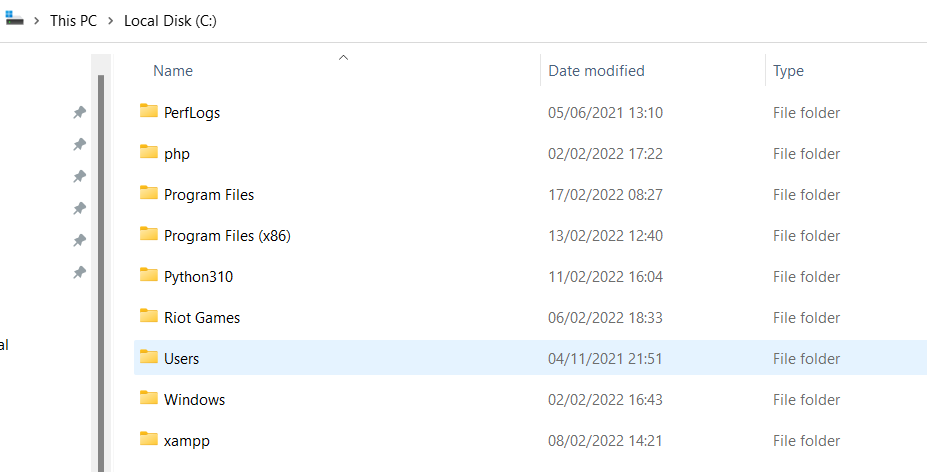
\includegraphics[width=0.7\textwidth,height=0.7\textheight,keepaspectratio]{images/root}
		\caption{Caminho onde se deve instalar o php}
		\label{phppath}
	\end{figure}

	A seguir terá de ativar as extensões para utilizar o postgresSQL no ficheiro "php.ini" que está dentro da pasta "php", como se pode ver no comando \ref{php.ini}. Para ativar basta retirar o ponto e vírgula e guardar o ficheiro.
	
		\begin{listing}[H]
		\begin{minted}{php}
		;extension=pdo\_odbc
		extension=pdo\_pgsql
		;extension=pdo\_sqlite
		extension=pgsql
		;extension=shmop
		\end{minted}
		\caption{Ativação das extensões no ficheiro php.ini}
		\label{php.ini}
		
	\end{listing}
	
	Posteriormente tem-se de criar uma variável de ambiente para que o sistema reconheça o php. Por isso na barra de pesquisa procure por "Editar variáveis de ambiente" e entre na aplicação. Deverá aparecer uma aplicação igual à da figura \ref{variveis}. 
	
	\begin{figure}[H] 
		\centering 
		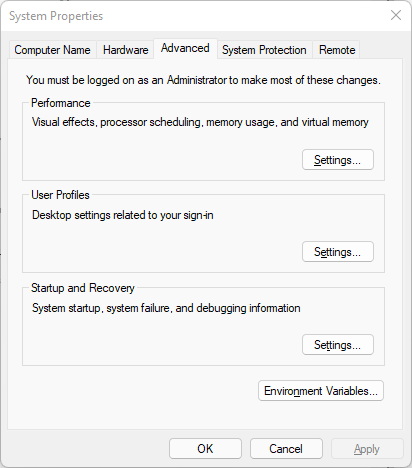
\includegraphics[width=0.7\textwidth,height=0.7\textheight,keepaspectratio]{images/editar}
		\caption{Aplicação para editar as variáveis de ambiente}
		\label{variveis}
	\end{figure}

	Depois clique em "Variáveis de Ambiente" e adicione uma nova variável tal como está apresentado nas figuras \ref{todasVariaveis} e \ref{pathphp}.
	
	\begin{figure}[H] 
		\centering 
		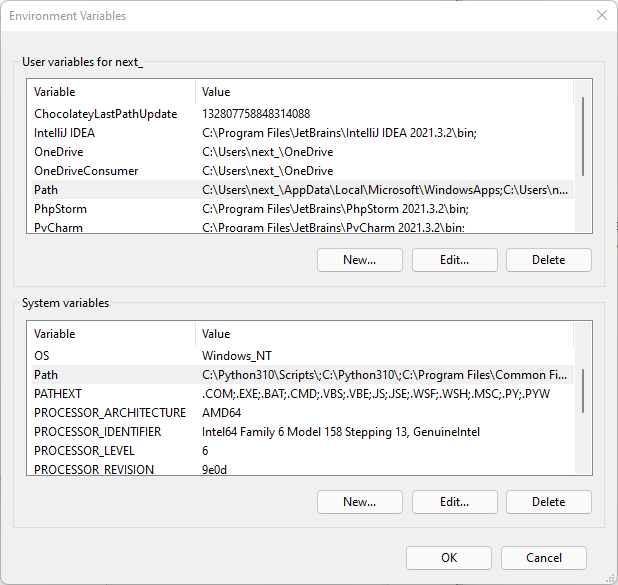
\includegraphics[width=0.7\textwidth,height=0.7\textheight,keepaspectratio]{images/todasvariaveis}
		\caption{Todas as variáveis de ambiente}
		\label{todasVariaveis}
	\end{figure}

	\begin{figure}[H] 
		\centering 
		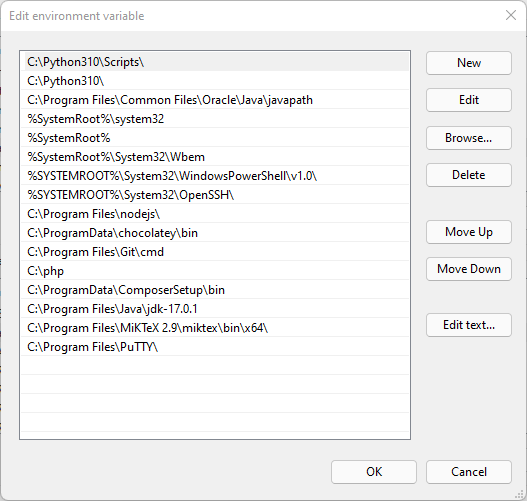
\includegraphics[width=0.7\textwidth,height=0.7\textheight,keepaspectratio]{images/pathphp}
		\caption{Aplicação para editar as variáveis de ambiente}
		\label{pathphp}
	\end{figure}

\section{Instalação do Composer}

Para instalar o composer no Windows basta descarregar o executável do \href{https://getcomposer.org/Composer-Setup.exe}{\underline{site oficial}}. Siga as orientações do instalador. Após terminada a instalação prossiga para a instalação do "Laravel".

\section{Instalação do Laravel}

Com o php e o composer instalado então pode-se instalar o Laravel. Para tal pode-se abrir uma janela da linha de comandos e digitar o comando \ref{laravel}.

	\begin{listing}[H]
	\begin{minted}{php}
	composer global require laravel/installer
	\end{minted}
	\caption{Comando para instalar laravel a partir do composer}
	\label{laravel}
	
\end{listing}

\chapter{Instalação da base de dados}

Como o site não funciona sem a base de dados configurada então irá ser criada uma base de dados local, utilizando PostgreSQL.

\section{Instalação do PostgreSQL}
Para instalar o "PostgreSQL" terá de baixar o executável que se encontra no \href{https://www.postgresql.org/download/windows/}{\underline{site}} e perseguir com as instruções. Durante a seleção de 
componentes, instale o “PostgreSQL Server”, “pgAdmin”, “StackBuilder” e “Command Line Tools”. 
Prossiga para a janela de diretório de dados (recomendamos os valores de defeito). Na próxima 
janela “Password”, escreva a password que servirá para o superuser “postgres”; não perca esta 
password. Prossiga para a janela “Port” e deixe a opção por defeito (5432). Siga para as restantes 
janelas e não altere os valores de defeito. O processo de instalação irá começar, pelo que deve 
esperar que este termine. No fim, desseleccione a caixa que pede para iniciar o “Stack Builder” e 
termine a instalação.

\section{Criação da base de dados}
Com o “PostgreSQL” instalado, pode criar uma base de dados. Para tal, inicie a aplicação 
“pgAdmin”, que irá abrir uma janela de browser e pedir para criar uma password; novamente, não 
se esqueça desta password. No lado esquerdo do ecrã, deve ter um browser de servers, expanda 
a listagem e escolha o seu servidor local (PostgreSQL xx). Expanda novamente, faça right-click e 
escolha ``Create Database…"

	Pode nomear a base de dados como quiser e clicar no “Save”. Com isto tem uma base dados 
	criada localmente. Agora é necessário preparar o Projeto para que use esta base de dados. 
	Na pasta do projeto ``calendario", navegue para o ficheiro .env e abra o seu conteúdo no editor 
	de texto da sua escolha. Dentro deste ficheiro irá encontrar as informações que o “Laravel” usa para 
	se conectar aos vários serviços que utiliza. De momento, só interessa alterar as informações 
	relativas à ligação à base de dados. Pode-se encontrar essas informações nas linhas que comecem 
	por DB.
	
	\begin{figure}[H] 
		\centering 
		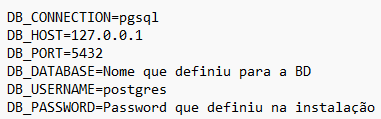
\includegraphics[width=0.7\textwidth,height=0.7\textheight,keepaspectratio]{images/env}
		\caption{Configuração do ficheiro env}
		\label{env}
	\end{figure}

\section{Migração das tabelas}
Por fim terá de criar todas as tabelas na base de dados utilizando o comando php artisan migrate --seed. E será colocados todos os cursos na base de dados.

\end{document}